\chapter{SegRanks - Proposed Manual Evaluation Method}

In this chapter we propose a novel manual evaluation method in which we create
a database of collected human annotations which can be reused later to
automatically evaluate similar, but yet unseen, translations or even to tune systems.
This method therefore lies on the boundary of automatic and manual evaluation
methods.

The proposed method consists of two parts which we describe and experiment with
in the following two sections. In the first section we describe the way of
collecting the database of humans judgements and report the human annotation
experiment which we conducted using the proposed method. In the second section
we present few methods which exploit the collected database: besides the
evaluation of annotated systems we experiment with extrapolating the database
to evaluate unseen translations and with tuning a machine translation system
using the database.

\section{Annotation of Short Segments}

In the WMT official human evaluation humans judge whole sentences. They get
five candidate translations of a given source sentence and their task is to
rank these candidates relatively (ties are allowed). One of disadvantages of
this method is that sentences are quite long and therefore quite hard to
remember for judge to compare them. Also when comparing longer sentences there
are much more aspects in which one sentence can be better or worse than second
sentence and therefore it is more difficult for judges to choose the better
candidate. 

\begin{algorithm}
    \begin{algorithmic}[1]
        %\Require{$x$ and $y$ are packed DNA strings of equal length $n$}
        \Function{ExtractSegments}{$treeNode, minLength, maxLength$}
            \Let{$extractedSegments$}{$list()$}
            \Let{$leaves$}{$treeNode.leaves()$}
            \If{$length(leaves) \le maxLength$}
                \If{$lenth(leaves) \ge minLength$}
                    \State $extractedSegments.append(leaves)$
                \EndIf
            \Else
                \For{$node$ \textbf{in} $treeNode.children()$  }
                \Let{$segments$}{\textsc{ExtractSegments}$(child, minLength, maxLength))$}
                \State $extractedSegments.extend(segments)$
                \EndFor
            \EndIf
            \Return $extractedSegments$
        \EndFunction
    \end{algorithmic}
    \caption{Short Segment Extraction From Source Side Parse Tree}
    \label{segment:extraction}
\end{algorithm}

To avoid these disadvantages we propose the following method. Instead of
judging whole sentences we extract shorter segments from candidates and give
them to judges to rank them. In order to extract meaningful segments with the
same meaning from all candidates we do the following procedure: First we parse
the source sentence and then we go recursively down the parsed tree and find
nodes which covers source segments with given maximum length (which is a
parameter of this method). This is exactly described in algorithm
\ref{segment:extraction}. Finally we project these extracted source segments to
their counterpart segments in all candidate sentences using an automatic
alignment.  You can find the whole process illustrated in figure \label{tree-align}
This extraction method is inspired by \perscite{human-in-the-loop}
and by the WMT07 manual evaluation \parcite{wmt-overview-2007}.

\begin{figure}
    \begin{center}
        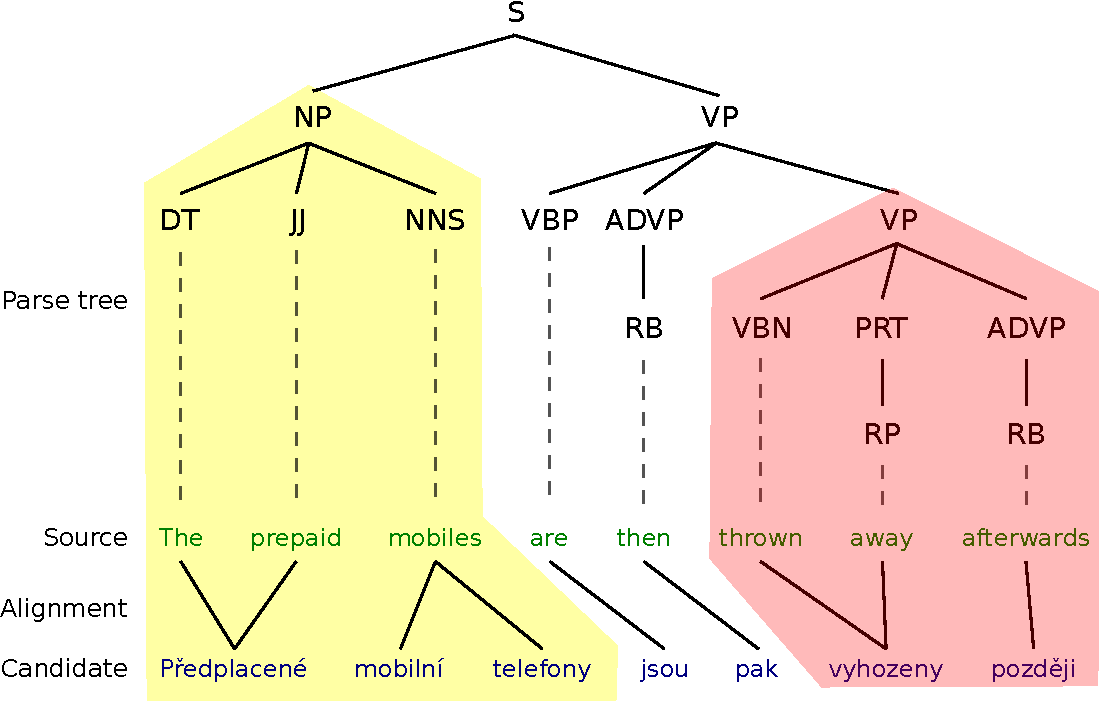
\includegraphics[width=\textwidth]{img/tree-align.pdf}
    \end{center}

    \caption[Candidate segments extraction process ilustrated]{You can see the
      candidate segments extraction process illustrated in this figure. For a
      given MT system, two segments were extracted from this sentence. The
      \pojem{maxLength} constant was set to the value 5 here to illustrate that
      not all words has to be covered by extracted segments.

}

    \label{tree-align}
\end{figure}

In the segment evaluation in \parcite{wmt-overview-2007}, these extracted
segments are only highlighted and shown to judges together with the rest of the
sentence.  Judges are asked to rank the highlighted segments in the context of
whole sentences.

We use different approach here which is more similar to that used in
\parcite{human-in-the-loop}. We show the extracted segments without any context
and ask judges to rank them. The only additional information provided to
annotators is the whole source sentence with the source segment highlighted.
Judges are told that they can imagine the rest of the sentence in which the
ranked segment fits best. They are instructed to penalize only those segments
for which they cannot imagine any appropriate rest of the sentence.

While we are aware that this approach has some disadvantages (which we
summarize bellow) there is one significant advantage: it is much more likely
that two systems produce the same translation of a short segment then they
would produce the same translation of a whole sentence. Because we do not show
the sentence context to annotators we can merge the equal segment candidates
into one, so the annotators have less candidate segments to rank. This also
allows us to reuse already collected human judgements later to evaluate a new
system which was not in the set of annotated systems (we present this
experiment in the section \ref{evaluating-new-systems}) or to tune parameters
of a system (we present this experiment in the section \ref{tuning-systems}).

The following list summarizes disadvantages of this method which we are aware
of. However, we believe that the advantages are still worth these
disadvantages and that we should still try it.

\begin{itemize}

  \item Annotators do not see the whole context of annotated short segments.
    For instance, the rest of the sentence of a given short candidate segment
    could require to have a noun in the segment in a particular grammatical
    case. Because annotators do not see this requirement, they cannot judge the
    candidate segment properly.  To partially remedy these two disadvantages we
    give all extracted short segments to annotators to judge at once, so they
    can at least imagine the context.

  \item This is very similar to the previous one. A system could translate
    shorter segments quite well but it can fail to combine them properly when
    creating the whole sentence translation. For instance a system may fail to
    preserve the subject -- verb agreement, which is very important in Czech.
    In their paper, \perscite{human-in-the-loop} suggest to go up the parse
    tree and extract also the longer segments which are consisted from already
    extracted shorter segments. However if we use this approach, the amount of
    annotation work would multiply few times. Furthermore, the longer segments
    are more difficult to rank and the chance that systems' candidates will be
    identicall (so that we can merge them for annotation) is lower.

  \item Extracted short segment candidates do not cover the whole sentence. For
    example in figure \label{tree-align} the words `jsou' and 'pak' are not
    part of any extracted segment. We would avoid this problem if we set the
    variable \pojem{minLength} to zero but it would generate high number of
    short segments to annotate. \XXX{Spocitat kolik, mozna ale v dalsi
    subsekci, mozna tam udelat i graf}

  \item Some segment candidates are much more important to convey the meaning
    than others and therefore should not have equal weight when interpreting
    them. When an annotator ranks system A better than system B in two of three
    ranked segments and system B better than system B in the third segment, it
    does not always mean that he would ranked system A better than system B
    when ranking whole sentences. The third segment could be much more
    significant for the quality of translation than the first two. We are
    afraid that it is not possible to easily avoid this problem. However, we
    also believe that this problem is not so serious and that possible
    differences in the importance of individual segments will be canceled out.

\end{itemize}

\subsection{Data and Segment Preparation}

We have conducted an annotation experiment using the proposed method. In this
section we describe what data we have used and how we prepare them for the
annotation experiment.

We used English to Czech part of the WMT14 \parcite{wmt14-overview-paper} test
set. We choose this data set to be able to compare experiments' results with
the official WMT14 human evaluation. 

The testset consists of 3003 sentences (68866 tokens). It contains both source
sentences and reference translations. Roughly a half of the sentences was
originally in Czech and was translated by human translators into English. The
second half of the sentences was translated in opposite direction. Besides the
source and reference translations, we also used candidate translations of 10
systems which participated in the WMT14 translation task. All systems are
listed in the table \ref{translation-task-participants}

\begin{table}[h]
  \small
  \begin{center}
    \begin{tabular}{|l|l|l|}
      \hline
      \textbf{ID} & \textbf{Type} & \textbf{Team} \\
      \hline
      \system{cu-depfix} & statistical & \multirow{4}{*}{Charles University, Prague \parcite{tamchyna2014}}  \\
      \system{cu-bojar} & statistical &  \\
      \system{cu-funky} & statistical &  \\
      \system{cu-tecto} & statistical &  \\
      \hline
      \system{uedin-phrase} & statistical &  \multirow{2}{*}{University of Edinburgh \parcite{durrani2014}} \\
      \system{uedin-uncnstr} &  statistical &  \\
      \hline
      \system{commercial-1} & rule-based & \multirow{2}{*}{Commercial machine translation systems} \\
      \system{commercial-2} & rule-based & \\
      \hline
      \system{online-a} & statistical & \multirow{2}{*}{Online statistical machine translation systems} \\
      \system{online-b} & statistical & \\
      \hline
    \end{tabular}
  \end{center}

  \caption[The MT systems which were used in the annotation experiment]{The
  machine translation systems participating in the WMT14 translation task in
  direction English-Czech which were used in the annotation experiment
  \XXX{Zkontrolovat typy nekterych systemu}}

  \label{translation-task-participants}
\end{table}

Source sentences and all candidate translations were tokenized using the script
\script{tokenizer.perl}. Unicode punctuation characters were normalized using
the script \script{replace-unicode-punctuation.perl}. (Both scripts are included
in the Moses toolkit).

The source sentences were parsed using the Stanford parser. We used
lexicalized \pojem{englishFactored} model \parcite{klein:factoredparser} which is
distributed with the parser. We have also tried unlexicalized \pojem{englishPCFG}
\parcite{klein:PCFGparser} and compare the segments extracted using the both parsers
on the small random sample of sentences. The \pojem{englishFactored} model yielded
subjectively better segments.

We computed an alignments between the source sentences and the candidate
translations using Giza++ \parcite{giza-pp}. Since the alignment algorithm is
unsupervised and the amount of all candidate translations is relatively small
($10 \times 3003$), we introduced more data by concatenating all candidate
translations with 646,605 sentences taken from Europarl parallel corpus
\parcite{koehn:europarl} and with 197,053 sentences taken from Czeng Corpus
\parcite{bojar:czeng}.  The concatenated parallel corpus was lowercased before
the alignment computation. 

We extracted short segments from the parsed source trees using the algorithm
\ref{segment:extraction}. The constant \pojem{minLength} was set to
the value 3 to filter out very short segments which are hard to judge without
context. This also helped to reduce the number of extracted segments to be
annotated. The constant \pojem{maxLength} was set to the value 6 so
the extracted segments were not too long to judge and in the same time it was
more likely that two candidate translations of a segment were equal and
therefore there would be less items to rank (our aim was to make annotations as
easy and fast as possible). We have experimented with various settings of these
two constants and the final settings seemed to generate reasonable number of
meaningful segments.

From 3003 source sentences, we have extracted 8485 segments of length 3 to 6
tokens. That is approximately 2.83 segments on a sentence on average. By
projecting the source segments to the candidate sentences using the computed
alignments, we got $10 \times 8485 = 84850$ candidate segments. However, after
the merging of equal segments only 50011 candidate segments left. This is 58.9
\% of the original candidate segments, or in other words, after the merging we
got 5.89 (instead of original 10) candidate segments to be ranked for each
source segment on average. These prepared candidate segments were inserted
into the database to be ranked by annotators.

\subsection{Segments Ranking}

We have developed a new annotation application for this annotation
project.\footnote{It would be probably possible to customize and use an
    existing annotation application, for example Appraise
    \parcite{mtmt12:appraise}.  However, since the ranking of short segments is
    quite specific it would require a lot of customization. We therefore
decided to develop our own light-weight web application which would suit our
needs perfectly and allow us to optimize efficiency of the annotation.} For
implementation details of this application, please see the chapter
\ref{implementation}.

You can find an example screen shot of this application in figure
\ref{segranks-screenshot}. Annotation instructions were displayed on each
annotation screen. This is an English translation of these instructions:

\begin{quote}
A number of segments are extracted from the annotated sentence. You are shown a
few candidate translations for each of these segments. Your task is to
distinguish the acceptable candidate translations (the meaning of the segment
can be guessed despite a few or more errors) from the unacceptable ones (the
meaning is definitely not possible to guess from the candidate segment). Also
please rank the acceptable candidate translations relatively from the best ones
to the worst ones.  Please, place better candidate translations higher, the
worser ones lower. You can place candidates of the same quality on the same
rank. Please place the unacceptable candidates to the position ``Garbage''

Please note that source segments and their candidate translations are chosen
automatically and does not have to be perfect. Consider them as only
approximate clue. If a candidate segment contains an extra word, which does not
correspond to the source segment but otherwise could be in the translated
sentence you do not have to consider such candidate as worser. If something is
missing in the candidate translation you should consider that as an error.
\end{quote}

Our goal was to make the annotation as efficient and user friendly as possible.
Annotators rank all the source segments of a sentence on a single screen (so
that they have to read the whole source sentence and reference translation only
once). For each annotated segment they see the source sentence repeated with
the annotated segment highlighted. Annotators rank the segment candidates by
drag-and-dropping them to appropriate rank positions. When all candidates of all
source segments of a sentence are ranked annotators are allowed to submit the
results to the server.  The web interface has responsive design, so it works
correctly on mobile devices.  The drag-and-drop works also on touch screens.
Annotators were therefore able to rank segments on a tablet.

\begin{figure}
    \begin{center}
        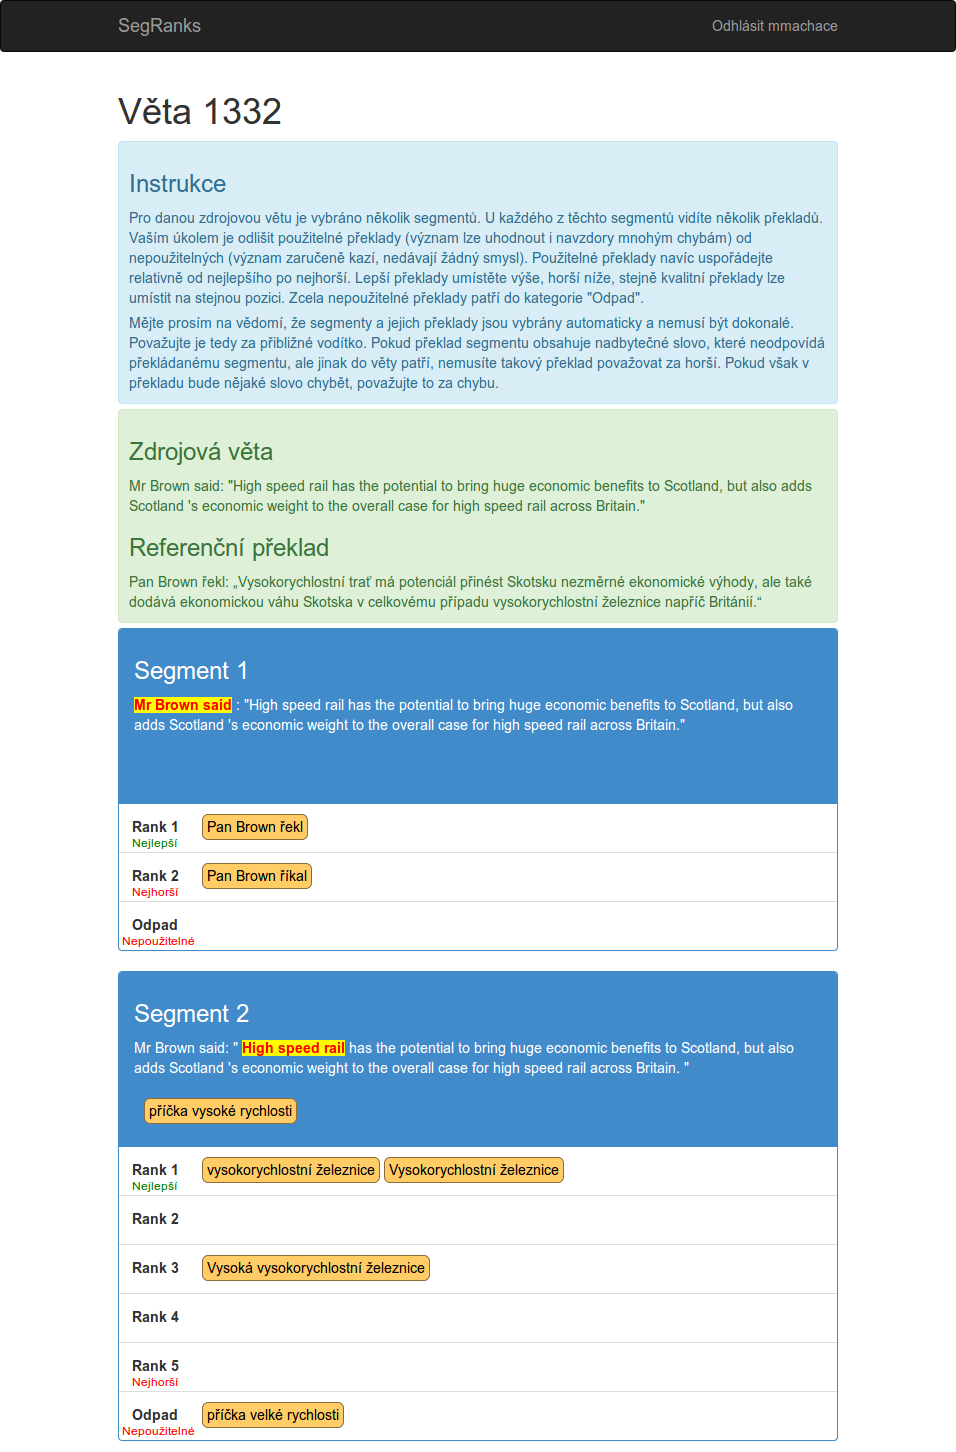
\includegraphics[width=\textwidth]{img/segranks-screenshot2.png}
    \end{center}
    \caption[A screen shot of the annotation application]{A screen shot of the
    annotation application. Annotators rank the candidate segments by dragging
and dropping them into the ranks.  Annotators see all annotated segments of a
sentence on a single screen}
    \label{segranks-screenshot}
\end{figure}

The very annotation experiment was conducted during May/June 2014. It lasted
exactly one month. During this time 17 annotators ranked segments of 2765
sentences, which is more than 92 \% of the prepared English-Czech test set.

\begin{table}
    \begin{center}
        \begin{tabular}{lrrrrrrr}
\textbf{ID} & \rotatebox{90}{\textbf{\#sentences}} & \rotatebox{90}{\textbf{\#segments}} & \textbf{time} & \rotatebox{90}{\textbf{reward/CZK}} & \rotatebox{90}{\textbf{annotatin-time/seconds}} & \rotatebox{90}{\textbf{kappa-intra}} & \rotatebox{90}{\textbf{kappa-inter}} \\
\hline
1 & 78 & 232 & 4:53:43 & 665 & 75 & 0.838 & 0.495 \\
4 & 87 & 248 & 5:00:46 & 711 & 74 & 0.283 & 0.145 \\
6 & 378 & 1160 & 16:53:13 & 3326 & 52 & 0.657 & 0.453 \\
7 & 243 & 663 & 11:16:26 & 1901 & 62 & 0.763 & 0.417 \\
8 & 6 & 20 & 0:21:06 & 57 & 63 \\
9 & 12 & 50 & 0:45:58 & 143 & 55 & 0.686 \\
10 & 98 & 274 & 5:04:45 & 785 & 66 & 0.673 & 0.320 \\
12 & 3 & 7 & 0:15:03 & 20 & 129 & 0.281 \\
13 & 424 & 1260 & 1 day, 2:26:14 & 3613 & 75 & 0.459 & 0.308 \\
15 & 106 & 282 & 5:17:58 & 808 & 67 & 0.611 & 0.401 \\
16 & 224 & 627 & 5:00:11 & 1797 & 28 & 0.655 & 0.614 \\
17 & 26 & 74 & 2:40:44 & 212 & 130 & 0.734 & 0.269 \\
18 & 83 & 234 & 7:02:10 & 670 & 111 & 0.676 & 0.385 \\
19 & 15 & 50 & 1:31:52 & 143 & 110 \\
21 & 483 & 1443 & 1 day, 13:44:37 & 4137 & 94 & 0.663 & 0.383 \\
22 & 117 & 338 & 6:00:36 & 969 & 64 & 0.714 & 0.431 \\
23 & 477 & 1371 & 22:07:35 & 3931 & 58 & 0.376 & 0.363 \\
\hline
   & 2773 & 8333 & 6 days, 14:22:57 & 23895 & 68 & 0.593 & 0.397 \\
        \end{tabular}
    \end{center}

    \caption[The list of annotators and their statistics]{The list of
        annotators and their statistics. The annotators are anonymized using
        their ID. The table contains the number of sentences annotated, the
        number of segments annotated, the time spend annotating, the reward in
    CZK, average time in seconds spend on one segment annotation and
intra-annotator and inter-annotator agreements. }

    \label{big-table}
\end{table}

\subsubsection{Annotator Agreements}

To measure reliability and robustness of the proposed annotation method we have
computed intra- and inter-annotator agreements. The reasonable degree of these
agreements supports the suitability of this method for machine translation
evaluation.

We measured the agreements using the Cohen's kappa coefficient ($\kappa$)
\parcite{cohen1960}. Let $P(A)$ be the proportion of times the annotators agree
and $P(E)$ be the proportion of time that they would agree by chance. Then the
Cohen's $\kappa$ is computed using the following formula:

\begin{equation*}
    \kappa = \frac{P(A)-P(E)}{1-P(E)}
\end{equation*}

\noindent Simply put, $\kappa$ is the proportion of times the annotators agrees
from all the times they would not agree by chance. Note that $\kappa$ is a
normalized version of $P(A)$, it considers how difficult it is to agree.
Values of $\kappa$ can be therefore compared across the various annotation
experiments. The maximum value is 1 which means that annotators always agree.
The zero value means that annotators agree as often as they would by chance.

In our case $P(A)$ and $P(E)$ are computed in context of pairwise comparisons.
Approximately 5 \% of the annotated sentences were annotated twice by two
different annotators (for the inter-annotator agreement).  Another 5 \% of the
sentences were annotated twice by the same annotator (for the intra-annotator
agreement). From all the segments of these double annotated sentences, we
extracted pairwise comparisons of candidate segments. Then we computed $P(A)$
as the proportion of pairwise comparisons in which two annotators agree (or one
annotator in different time in the case of intra-annotator agreement). 

Finally we computed $P(E)$ as 

\begin{equation*}
    P(E) = P(A>B)^2 + P(A=B)^2 + P(A<B)^2
\end{equation*}

\noindent where $P(A>B)$, $P(A=B)$ and $P(A<B)$ were computed empirically. The
value of $P(E)$ in our experiment is 0.394, which means that the probability of
the outcomes $A>B$, $A=B$ and $A<B$ is not uniform.

The final values of inter-annotator and intra-annotator $\kappa$ can be found
in the table \ref{agreements} together with corresponding $\kappa$ values from
WMT14 translation task.  \parcite{wmt14-overview-paper} computed similarly on
the same testset for comparisons.  The exact interpretation of the kappa
coefficient is difficult, but according to \cite{landis77}, 0 -- 0.2 is slight,
0.2 -- 0.4 is fair, 0.4 -- 0.6 is moderate, 0.6 -- 0.8 is substantial and 0.8
-- 1.0 is almost perfect.  You can see that we get both $\kappa$ scores better
than they are in WMT14. However, they are still quite poor and we expected them
to be higher, since the annotation task was designed to be much simpler than
the official WMT human evaluation.

We also computed the agreements $\kappa$ for
individual annotators and report them in the table \ref{big-table}.  As you can
see, these scores are varying a lot. Based on these scores we could filter out
unreliable annotators. However we do not do that to have the experiment
comparable to the WMT14 experiment.


\begin{table}
    \begin{center}
        \begin{tabular}{r|cc}
                                     & our method & \cite{wmt14-overview-paper} \\
            \hline
            intra-annotator $\kappa$ &  0.593     & 0.448    \\
            inter-annotator $\kappa$ &  0.397     & 0.360     \\
        \end{tabular}
    \end{center}

    \caption[Inter-annotator and intra-annotator $\kappa$ scores]{$\kappa$
        scores measuring intra-annotator and inter-annotator agreements. We
        also report corresponding $\kappa$ scores from official WMT translation
        task for comparison.  Please see the table \ref{big-table} for the
    annotator agreements computed for individual annotators}

    \label{agreements}
\end{table}




\section{Experiments}

In this section we describe several experiments with the collected database of
annotations. 

\subsection{Overall Ranking of Annotated Systems}
\label{evaluating-annotated-systems}

In the first experiment we would like to show that the proposed method can be
used to produce overall ranking of the annotated systems which will be very
similar to the official human evaluation in WMT with much less human effort
\XXX{dolozit, pokud je to vubec pravda a pokud to vubec pujde}.

The obtained database contains a list of annotations for each extracted source
segment from each source sentence. A list can be empty (not all of the
sentences were annotated), it can contain more than one annotation (some
segments were annotated twice by an annotator, some segments were annotated by
multiple annotators), but most of the time it contains only one annotation.

An annotation is a mapping from the set of candidate segments to the set of
ranks ${1 \ldots N+1}$, where $N$ is the count of unique candidate segments.
(To discriminate the relative quality of all segments, annotators had available
$N$ ranks which could be all occupied when there are no ties. The rank $N+1$
represents the ``garbage'' category from the annotation application. However in
all of our experiments reported in this thesis we consider this category as one
more, the worst, rank). A Lower rank of a segment means that the candidate
segment was ranked better. This is an example \metoda{segment annotation} of a
source segment ``the huge volume'':

\begin{verbatim}
    {
      'velkému objemu' : 1,
      'obrovské hlasitosti' : 5,
      'obrovský objem' : 2,
      'obrovské množství' : 2,
    }
\end{verbatim}

We expanded these segment annotations with the information about the systems
which produced the segments. The ranks in the annotations are now indexed by
the system names.  If more systems translated a source segment as the same
candidate segment the candidate segment's rank is copied to all the systems.
This is the time when we use advantage of ranking short segments which are
often translated identically.  The following is the \metoda{system annotation}
after expansion of the above \metoda{segment annotation}:

\begin{verbatim}
    {
      'uedin-unconstrained.3424' : 2,
      'commercial1.3556' : 5,
      'commercial2.3222' : 2,
      'CU-TectoMT.2950' : 1,
      'onlineB.0' : 2,
      'onlineA.0': 2,
      'cu-funky.3515' : 2,
      'cu-bojar.3483' : 2,
      'uedin-wmt14.3021': 2,
      'cu-depfix.3452': 2
    }
\end{verbatim}

These rankings are now very similar to those obtained in the official WMT human
evaluation. These annotations are mostly interpreted as pairwise systems'
comparisons (for each combination of size 2 of all systems we have a pairwise
comparison), where the absolute values of the ranks and their absolute
differences between them are not considered. From above \metoda{system
annotation}, the following \metoda{pairwise comparisons} are be extracted (only
a few extracted pairwise comparisons are listed here for the sake of brevity,
generally $N \times (N-1) / 2$ pairwise comparisons are extracted, where $N$ is
number of all systems):

\begin{verbatim}
    [
      'uedin-unconstrained.3424' < 'commercial1.3556',
      'uedin-unconstrained.3424' = 'commercial2.3222',
      'uedin-unconstrained.3424' > 'CU-TectoMT.2950',
      ...
      'commercial1.3556' > 'commercial2.3222',
      'commercial1.3556' > 'CU-TectoMT.2950',
      ...
    ]
\end{verbatim}

The interpretation of these pairwise comparisons was changed several times
during the WMT workshops. Here, we use \metoda{Ratio of wins (ignoring ties)}
method, which was introduced by \perscite{bojar:grain:of:salt} and used in
WMT12 workshop \parcite{callisonburch:wmt12}. This method is based on a method
used in several WMT workshops before WMT12 and it is quite easy to compute and
interpret results.

For a given set $C$ of segment-level extracted pairwise comparisons
$(s_1,s_2,c)$, where 

\begin{equation*}
c = \begin{cases}
  win  & \text{if $rank(s_1) < rank(s_2)$} \\
  loss & \text{if $rank(s_1) > rank(s_2)$} \\
  tie  & \text{if $rank(s_1) = rank(s_2)$} \\
    \end{cases}
\end{equation*}

\noindent we define for each system $s$ the total number of wins, losses and ties:

\begin{equation*}
\begin{array}{rcl} 
  win(s)  & := & |\{(s,\bar{s},c) \in C; c = win\}| + |\{(\bar{s},s,c) \in C; c = loss\}| \\
  loss(s) & := & |\{(s,\bar{s},c) \in C; c = loss\}| + |\{(\bar{s},s,c) \in C; c = win\}| \\
  ties(s) & := & |\{(s,\bar{s},c) \in C; c = tie\}| + |\{(\bar{s},s,c) \in C; c = tie\}| \\
\end{array}
\end{equation*}

Then the \metoda{Ratio of wins (ignoring ties)} is computed using the following formula:

\begin{equation*}
  E_{win}(s) = \frac{win(s)}{win(s) + loss(s)} 
\end{equation*}

\begin{table}
  \begin{center}
    \subfloat[Short segments judgements]{
      %\begin{center}
        \begin{tabular}{|l|c|}
          \hline
          \textbf{System} & \textbf{Score} \\
          \hline
           cu-depfix           &  0.5777 \\
           onlineB             &  0.5642 \\
           uedin-unconstrained &  0.5626 \\
           cu-bojar            &  0.5606 \\
           cu-funky            &  0.5566 \\
           uedin-wmt14         &  0.5498 \\
           onlineA             &  0.5007 \\
           CU-TectoMT          &  0.4485 \\
           commercial1         &  0.3992 \\
           commercial2         &  0.3492 \\
          \hline
        \end{tabular}
      %\end{center}
      \label{all-systems-segranks-results}
    }
    \subfloat[Official WMT14 judgements]{
      %\begin{center}
        \begin{tabular}{|l|c|}
          \hline
          \textbf{System} & \textbf{Score} \\
          \hline
          cu-depfix          &  0.6101 \\
          cu-bojar           &  0.6011 \\
          uedin-unconstrained&  0.5967 \\
          cu-funky           &  0.5823 \\
          onlineB            &  0.5439 \\
          uedin-wmt14        &  0.5285 \\
          onlineA            &  0.5039 \\
          CU-TectoMT         &  0.4473 \\
          commercial1        &  0.3617 \\
          commercial2        &  0.2780 \\
          \hline
        \end{tabular}
      \label{all-systems-wmt-results}
    }

  \end{center}

  \caption{Overall rankings of systems according to \metoda{Ratio of wins
  (ignoring ties)} score. You can see the results computed on both short
segments judgements and on official WMT14 human judgements side by side to
compare the differences.}

  \label{all-systems-results}
\end{table}

\subsubsection{Results}

The overall ranking of systems, which participated in WMT14 Translation Task in
English-Czech direction, according to the \metoda{Ratio of wins (ignoring
ties)} computed on the short segments judgements is reported in the table
\ref{all-systems-segranks-results}.

To compare our method with the classic method of judging whole sentences, we
have also computed the \metoda{Ratio of wins (ignoring ties)} on the judgements
collected during WMT14 manual evaluation. You can see these results in the
table \ref{all-systems-wmt-results}.

You can notice that the range of scores computed on the short segments
judgements is much narrower (0.35 --- 0.58) than the range of scores computed
on the sentence judgements (0.28 --- 0.61). This can be explained by the
following: If system A beats system B in a sentence-level judgement of a
particular sentence it does not necessarily mean that in segment-level judging
system A will be better than system B on all segments of the sentence. System A
will be probably better on a majority of the segments (but even that does not
have to be always true). When computing the ratio of wins on the sentence-level
judgements, system A gets one win and system B gets one loss. However, when
computing the ratio of wins on the segment-level system A gets for example two
wins and one loss, system B one win and two losses. It should be clear now that
computing expected wins on the sentence-level judgements is coarser while our
method is more fine-grained.  \XXX{Co z toho vlastne plyne? Je to dobre, nebo
spatne?}

The overall rankings of systems obtained by both of the methods is very
similar. However, there are two changes when comparing to the sentence-level
judgments results: system online-B is better and system cu-bojar is worser
according to the segments-level judgments results. We try to explain this in the Analysis.

\subsubsection{Analysis}

To see the difference between the segment-level judgements and sentence-level
judgements we have computed Kendall tau rank correlation coefficient, also
known as Kendall's $\tau$, between segment-level pairwise comparisons and
sentence-level pairwise comparisons. This coefficient is used to measures how
often a set of pairwise rankings agrees with another set of pairwise rankings.
The basic formula for Kendall's $\tau$ is:

\begin{equation*}
  \tau = \frac{|Concordant| - |Discordant|}{|Concordant| + |Discordant|}
\end{equation*}

\noindent where $Concordant$ is the set of pairwise combination where both sets
of pairwise rankings agrees with each other and $Discordant$ is the set of
pairwise combination where the sets do not agree in pairwise ranking.
\XXX{mozna vyhodit predchozi vetu}  We will discuss the Kendall's $\tau$ in
more details in chapter \ref{metrics}. Here we computed $|Concordant|$ as the
number of pairwise segment-level judgments which agrees with the corresponding
sentence-level judgment. Similarly, $|Discordant|$ is the number of those which
does not agree with the corresponding sentence-level judgment. In this section
we does not consider any tied pairwise comparisons.

\begin{table}
  \begin{center}
    \subfloat[Better systems]{
      %\begin{center}
        \begin{tabular}{|l|c|}
          \hline
          \textbf{System}                   &   $\tau$ \\
        \hline
         cu-funky            &        0.428 \\
         cu-depfix           &        0.405 \\
         onlineB             &        0.398 \\
         cu-bojar            &        0.394 \\
         uedin-uncon. &        0.390 \\
         uedin-wmt14         &        0.363 \\
         onlineA             &        0.312 \\
         CU-TectoMT          &        0.270 \\
         commercial1         &        0.166 \\
         commercial2         &        0.123 \\
          \hline
        \end{tabular}
      %\end{center}
      \label{sentence-segments-judgments-correlations-better}
    }
    \subfloat[Worse systems]{
      %\begin{center}
        \begin{tabular}{|l|c|}
          \hline
          \textbf{System}                   &   $\tau$ \\
       \hline
         commercial2         &        0.492 \\
         commercial1         &        0.441 \\
         CU-TectoMT          &        0.385 \\
         onlineA             &        0.328 \\
         uedin-uncon. &        0.260 \\
         uedin-wmt14         &        0.257 \\
         cu-funky            &        0.230 \\
         cu-bojar            &        0.227 \\
         cu-depfix           &        0.225 \\
         onlineB             &        0.225 \\
          \hline
        \end{tabular}
      \label{sentence-segments-judgments-correlations-worse}
    }
    
    \subfloat[All systems]{
      %\begin{center}
        \begin{tabular}{|l|c|}
          \hline
          \textbf{System}                   &   $\tau$ \\
        \hline
         commercial2         &        0.394 \\
         cu-funky            &        0.348 \\
         commercial1         &        0.345 \\
         uedin-uncon. &        0.341 \\
         cu-depfix           &        0.335 \\
         CU-TectoMT          &        0.333 \\
         cu-bojar            &        0.328 \\
         onlineB             &        0.321 \\
         onlineA             &        0.320 \\
         uedin-wmt14         &        0.317 \\
          \hline
        \end{tabular}
      \label{sentence-segments-judgments-correlations-all}
    }

  \end{center}

  \caption{Kendall's $\tau$ correlations between the segment-level and
    sentence-level judgments. For a given system we computed the correlation on
    all pairwise comparisons including the given system. The table
    \ref{sentence-segments-judgments-correlations-better} contains correlations
    computed on sentence-level judgments where the given system was better, the
    table \ref{sentence-segments-judgments-correlations-worse} is computed on
    sentence-level comparisons where the given system was worse and finally the
  table \ref{sentence-segments-judgments-correlations-all} was computed on all
pairwise comparisons including the system. The systems are sorted by the
correlation in reverse order.} 

  \label{sentence-segments-judgments-correlations}
\end{table}

The computed correlation are tabulated in the table
\ref{sentence-segments-judgments-correlations}. The order of systems in the
table \ref{sentence-segments-judgments-correlations-better} is quite similar to
the order of systems in the overall rankings (table \ref{all-systems-results});
better systems have higher correlation than worse systems. This is somehow
expected: systems whose segments were ranked more often better are more likely
to be ranked better on sentence-level. You can also read the table in the
following way: If a sentence of system cu-funky was ranked better on
sentence-level it is very likely (71\%) that the segments of the sentence were
ranked better also. On the other hand, if system commercial2 was ranked better
on sentence-level only a little more than half of the segments were ranked
better also. The table \ref{sentence-segments-judgments-correlations-worse} is
similar but in reversed order.

The influence of a system's quality should be canceled out in the table
\ref{sentence-segments-judgments-correlations-all}. You can see, that systems
cu-bojar and onlineB have the Kendall's $\tau$ lower (although not the lowest).
This together with the fact that both systems lies in a cluster of systems of
very similar quality is consistent with their change in the overall ranking of
systems. This, however, does not explain that.

For the explanation of the differences between the overall rankings computed on
sentence-level and segment-level judgments we have to look into the data. We
want to find candidate translations for wich the sentence judgments disagree as
much as possible with the segment judgments. To quantify this property we have
defined \metoda{disagreement quotient}:

\begin{equation*}
  q_d(s,n) = \frac{
    win_{seg}(s,n) / (win_{seg}(s,n) + loss_{seg}(s,n))
  }{
    win_{sent}(s,n)/(win_{sent}(s,n) + loss_{sent}(s,n))
  }
\end{equation*}

\noindent where $s$ is a system, $n$ is a sentence number, $win_{seg}(s,n)$ is
the number of segment-level comparisons where the $n$-th candidate sentence
translated by system $s$ won and $loss_{sent}(s,n)$ is the number of
comparisons in which the candidate sentence losses. Finally, $win_{sent}(s,n)$
and $loss_{sent}(s,n)$ are defined similarly for the sentence-level
comparisons.

Using this measure we found candidate sentence translations with the highest
\metoda{disagreement quotient} and tried to analyze the cause of the
disagreement between the sentence-level and segment-level judgments. In the
following we present a few of these sentences with comments. The extracted
segments which were ranked are bolded.

\begin{quote}
  Letecké linky začaly nabíjení pro \textbf{první a druhý odbavených zavazadel} v roce 2008. (Sentence 715, online-B)
\end{quote}

The translation of the segment is relatively good, the case of the noun phrase
is wrong but the meaning could be understood. The reason why the whole sentence
was ranked poorly is probbably the word ``nabíjení'', which is obviously a
wrong lexical choice of the MT system. Unfortunately this word is not covered
by the only ranked segment.



%\ref{sentence-segments-judgments-correlations-worse} is somehow expected. The orde



\XXX{Vybrat nejake dve vety, kde budou nejvetsi rozdily mezi sentence-level a
segment level judgements}

\subsection{Evaluating New Systems}
\label{evaluating-new-systems}

\XXX{Zde zkusim pouzit vytvorenou databazi pro vyhodnoceni noveho systemu}

\XXX{provest experimenty podobne tem z clanku An Evaluation Tool for Machine
Translation: Fast Evaluation for MT Research}

\subsection{Tuning Systems}
\label{tuning-systems}

\XXX{Zde zkusim pouzit vytvorenou databazi pro MT tuning}

\section{Comparison to Other Manual Methods}
